% !TEX root = main.tex
\documentclass[12pt,a4paper,oneside]{report}

% Compilar desde esta carpeta con pdfLaTeX (latexmk), LuaLaTeX o XeLaTeX.
\usepackage[spanish,es-nodecimaldot]{babel}
\usepackage{iftex}
\ifPDFTeX
    \usepackage[T1]{fontenc}
    \usepackage[utf8]{inputenc}
    \usepackage{lmodern}
    \usepackage{textcomp}
    \usepackage{eurosym}
    \DeclareUnicodeCharacter{20AC}{\euro}
\else
    \usepackage{fontspec}
\fi
\usepackage{geometry}
\usepackage{graphicx}
\usepackage[inkscapelatex=false]{svg}
\usepackage{float}
\usepackage{booktabs}
\usepackage{tabularx}
\usepackage{array}
\usepackage{hyperref}
\usepackage{xurl}
\usepackage{enumitem}
\usepackage{microtype}
\usepackage{xcolor}
\usepackage{pdflscape}

\definecolor{urjcred}{RGB}{186, 12, 47}
\definecolor{urjcslate}{RGB}{75, 85, 99}

\geometry{margin=2.5cm}
\setlength{\parskip}{0.45em}
\setlength{\parindent}{0pt}
\hypersetup{colorlinks=true,linkcolor=black,urlcolor=blue,citecolor=black}
\renewcommand{\arraystretch}{1.2}

\title{Diseño y Arquitectura del Software\\[0.5em]
\large Práctica 1: Arquitectura de un periódico digital}
\author{Grupo 5 -- Antonio Machuca, Enrique Aldama, Sergio González, Sara Guillén, David Sticea, Elena Romera}
\date{Curso académico 2026--2027}

\begin{document}

\begin{titlepage}
    \centering
    \vspace*{0.1cm}
    \includesvg[width=3.6cm]{assets/Logo_URJC.svg}\par
    \vspace{0.45cm}
    {\scshape\large Universidad Rey Juan Carlos\par}
    \vspace{0.1cm}
    {\color{urjcslate}\normalsize Escuela Técnica Superior de Ingeniería Informática\par}
    {\color{urjcslate}\small Grado en Ingeniería del Software\par}

    \vspace{0.85cm}
    {\color{urjcred}\rule{\textwidth}{1.6pt}}\par
    \vspace{0.45cm}
    {\large\bfseries\color{urjcslate} DISEÑO Y ARQUITECTURA DEL SOFTWARE (DAS)\par}
    \vspace{0.3cm}
    {\Huge\bfseries Práctica 1\par}
    \vspace{0.2cm}
    {\Large Captura y Representación de Decisiones de Diseño:\\[0.15em]
    Sistema de Periódico Digital\par}
    \vspace{0.45cm}
    {\color{urjcred}\rule{\textwidth}{0.7pt}}\par

    \vfill
    {\color{urjcslate}\normalsize Móstoles, Madrid\par}
    \vspace{0.12cm}
    {\bfseries Curso académico 2026--2027\par}
\end{titlepage}

\pagenumbering{roman}
\tableofcontents
\clearpage
\pagenumbering{arabic}

% Capítulos estructurados de la memoria.
\chapter{Introducción y análisis de requisitos}

\section{Descripción del trabajo}

El objetivo de esta práctica es diseñar la arquitectura software de un periódico digital a partir del caso de estudio.

Para ello, hemos analizado los requisitos funcionales y de dominio, planteado diferentes decisiones arquitectónicas y representado las soluciones mediante diagramas UML de clases y paquetes.

El sistema que tenemos que diseñar cuenta con las siguientes funcionalidades:

\begin{itemize}[leftmargin=*]
    \item Una interfaz web responsiva para PC y Tablet.
    \item Suscripción y baja anónima a noticias de política, economía, sociedad, nacionales e internacionales.
    \item Tres modalidades de suscripción: trimestral (70~€), semestral (130~€) y anual (190~€).
    \item Gestión de pagos mediante Stripe, permitiendo hasta tres reintentos cuando falla un pago.
    \item Estadísticas de uso para administradores y redactores.
    \item Dos bases de datos PostgreSQL 19: una para administradores y redactores y otra para suscriptores.
\end{itemize}

Durante el desarrollo de la práctica hemos tenido que revisar algunas de las decisiones iniciales, ya que no todas las soluciones propuestas eran correctas para cumplir todos los requisitos y construir la arquitectura que buscábamos. Por eso, las discusiones entre arquitectos senior y cognitivos han sido una parte importante del trabajo. Nos han permitido cuestionar las decisiones, comparar alternativas y corregir algunos problemas antes de continuar con el diseño UML.

\section{Análisis de requisitos}

\subsection{Requisitos funcionales}

En el archivo \href{Requisitos/REQUISITOS.xlsx}{REQUISITOS.xlsx} hemos recogido los seis requisitos funcionales principales del sistema.

\begin{table}[H]
\centering
\small
\begin{tabularx}{\textwidth}{@{}p{0.08\textwidth}p{0.24\textwidth}X@{}}
\toprule
\textbf{ID} & \textbf{Nombre} & \textbf{Descripción} \\
\midrule
RF1 & Discriminación del cliente & El sistema debe distinguir entre los clientes PC y Tablet. \\
RF2 & Suscripción y baja anónima & Los lectores pueden suscribirse y darse de baja de las diferentes categorías de noticias de forma anónima. \\
RF3 & Modalidades de suscripción & El sistema permite seleccionar suscripciones trimestrales, semestrales y anuales con sus correspondientes importes. \\
RF4 & Cobro externalizado & El sistema debe realizar los cobros mediante una pasarela externa. \\
RF5 & Reintentos de pago & Cuando falla un pago, el sistema debe permitir reintentarlo hasta tres veces. \\
RF6 & Estadísticas de uso & Los administradores y redactores pueden consultar las noticias más leídas, el tiempo de permanencia, las tasas de rebote y las conversiones a suscriptores. \\
\bottomrule
\end{tabularx}
\caption{Requisitos funcionales del sistema.}
\label{tab:requisitos-funcionales}
\end{table}

\subsection{Requisitos de dominio}

También hemos identificado tres requisitos de dominio.

\begin{table}[H]
\centering
\small
\begin{tabularx}{\textwidth}{@{}p{0.08\textwidth}p{0.27\textwidth}X@{}}
\toprule
\textbf{ID} & \textbf{Nombre} & \textbf{Descripción} \\
\midrule
RD1 & Uso de Stripe & La pasarela de pago utilizada debe ser Stripe. \\
RD2 & Comunicación HTTP/REST & Las peticiones entre el frontend y el backend deben realizarse mediante HTTP/REST. \\
RD3 & Bases de datos PostgreSQL 19 & El sistema debe utilizar dos bases de datos PostgreSQL 19, una para administradores y redactores y otra para suscriptores. \\
\bottomrule
\end{tabularx}
\caption{Requisitos de dominio del sistema.}
\label{tab:requisitos-dominio}
\end{table}

\subsection{Revisión de los requisitos iniciales}

Durante el análisis inicial planteamos algunos requisitos adicionales porque considerábamos que podían ser necesarios para el funcionamiento del periódico. Sin embargo, después de revisar el enunciado, comprobamos que algunos no estaban bien justificados, dado que los habíamos sacado del contexto y no correspondían a requisitos solicitados en el caso de estudio. Por este motivo, revisamos los requisitos y mantuvimos los relacionados con las funcionalidades y restricciones que teníamos que resolver. Esta revisión fue importante para poder realizar adecuadamente la práctica.

\chapter{Semana 1: análisis de requisitos y selección del estilo arquitectónico}

Durante la primera semana de la práctica se realizó el análisis de los requisitos funcionales y de dominio del periódico digital y se comenzó a definir su arquitectura software. En esta primera fase se plantearon distintas alternativas para organizar el sistema, comenzando con una propuesta monolítica que posteriormente fue revisada y sustituida por una arquitectura cliente-servidor con API REST.

Las decisiones correspondientes a esta primera semana quedaron estudiadas en las ADR-0001.1, ADR-0001.2 y ADR-0001.3.

\section{Decisión inicial: arquitectura monolítica}

En la primera decisión arquitectónica, \href{Decisiones/0001.1-seleccion-estilo-arquitectonico-global.md}{ADR-0001.1}, los arquitectos senior propusieron una arquitectura monolítica basada en MVC. Esta primera opción permitía organizar la presentación, la lógica de negocio y el acceso a datos dentro de una misma aplicación. Se consideró inicialmente por su sencillez y porque permitía establecer una primera estructura para las funcionalidades del periódico.

Sin embargo, durante la revisión realizada por los arquitectos cognitivos se plantearon dudas sobre la separación entre la interfaz web y la lógica de negocio. Se cuestionó la utilidad de mantener ambas responsabilidades dentro de una misma aplicación, además de la necesidad de diferenciar mejor la parte de presentación de los servicios del backend para organizar las suscripciones, los pagos mediante Stripe y las estadísticas.

A partir de estas observaciones, los arquitectos senior revisaron la propuesta y volvieron a valorar las alternativas arquitectónicas.

\section{Revisión de las alternativas y cambio de arquitectura}

Durante la revisión se consideraron las alternativas recogidas en las decisiones arquitectónicas: una arquitectura monolítica basada en MVC, una arquitectura cliente-servidor con API REST, una arquitectura orientada a servicios (SOA) y una arquitectura de microservicios orientada a eventos.

La propuesta monolítica inicial permitía mantener una estructura sencilla, pero se consideró que una arquitectura cliente-servidor representaba mejor la separación entre el frontend web y el backend que se buscaba para este sistema.

En cuanto a SOA, se descartó porque la incorporación de un bus de servicios y una estructura de integración más amplia añadía demasiada complejidad para lo que se pedía. La alternativa de microservicios también se descartó, ya que suponía dividir el periódico en diferentes servicios independientes y gestionar su comunicación.

Finalmente, se eligió una arquitectura cliente-servidor con API REST. Esta opción permite diferenciar la interfaz utilizada por los lectores de los servicios encargados de gestionar las funcionalidades del periódico y establecer la comunicación HTTP/REST indicada en el requisito RD2.

Tras esta revisión, se documentó la anulación de la propuesta inicial en la \href{Decisiones/0001.2-anulacion-decision-0001.1.md}{ADR-0001.2}. La nueva solución quedó recogida en la \href{Decisiones/0001.3-migracion-estilo-cliente-servidor-api-rest.md}{ADR-0001.3}.

\section{Arquitectura cliente-servidor con API REST}

La arquitectura seleccionada establece una separación entre el frontend web, encargado de la presentación e interacción con los lectores, y el backend, donde se encuentran los servicios relacionados con las noticias, las suscripciones, la facturación y las estadísticas. El frontend debe permitir el acceso desde PC y Tablet, mientras que el backend se encarga de procesar las peticiones y gestionar las operaciones del sistema. La comunicación entre ambas partes se realiza mediante HTTP/REST, como se establece en el requisito RD2.

\section{Representación de la arquitectura en UML}

Según la primera propuesta, los arquitectos junior elaboraron un diagrama UML basado en la arquitectura monolítica.

\begin{figure}[H]
    \centering
    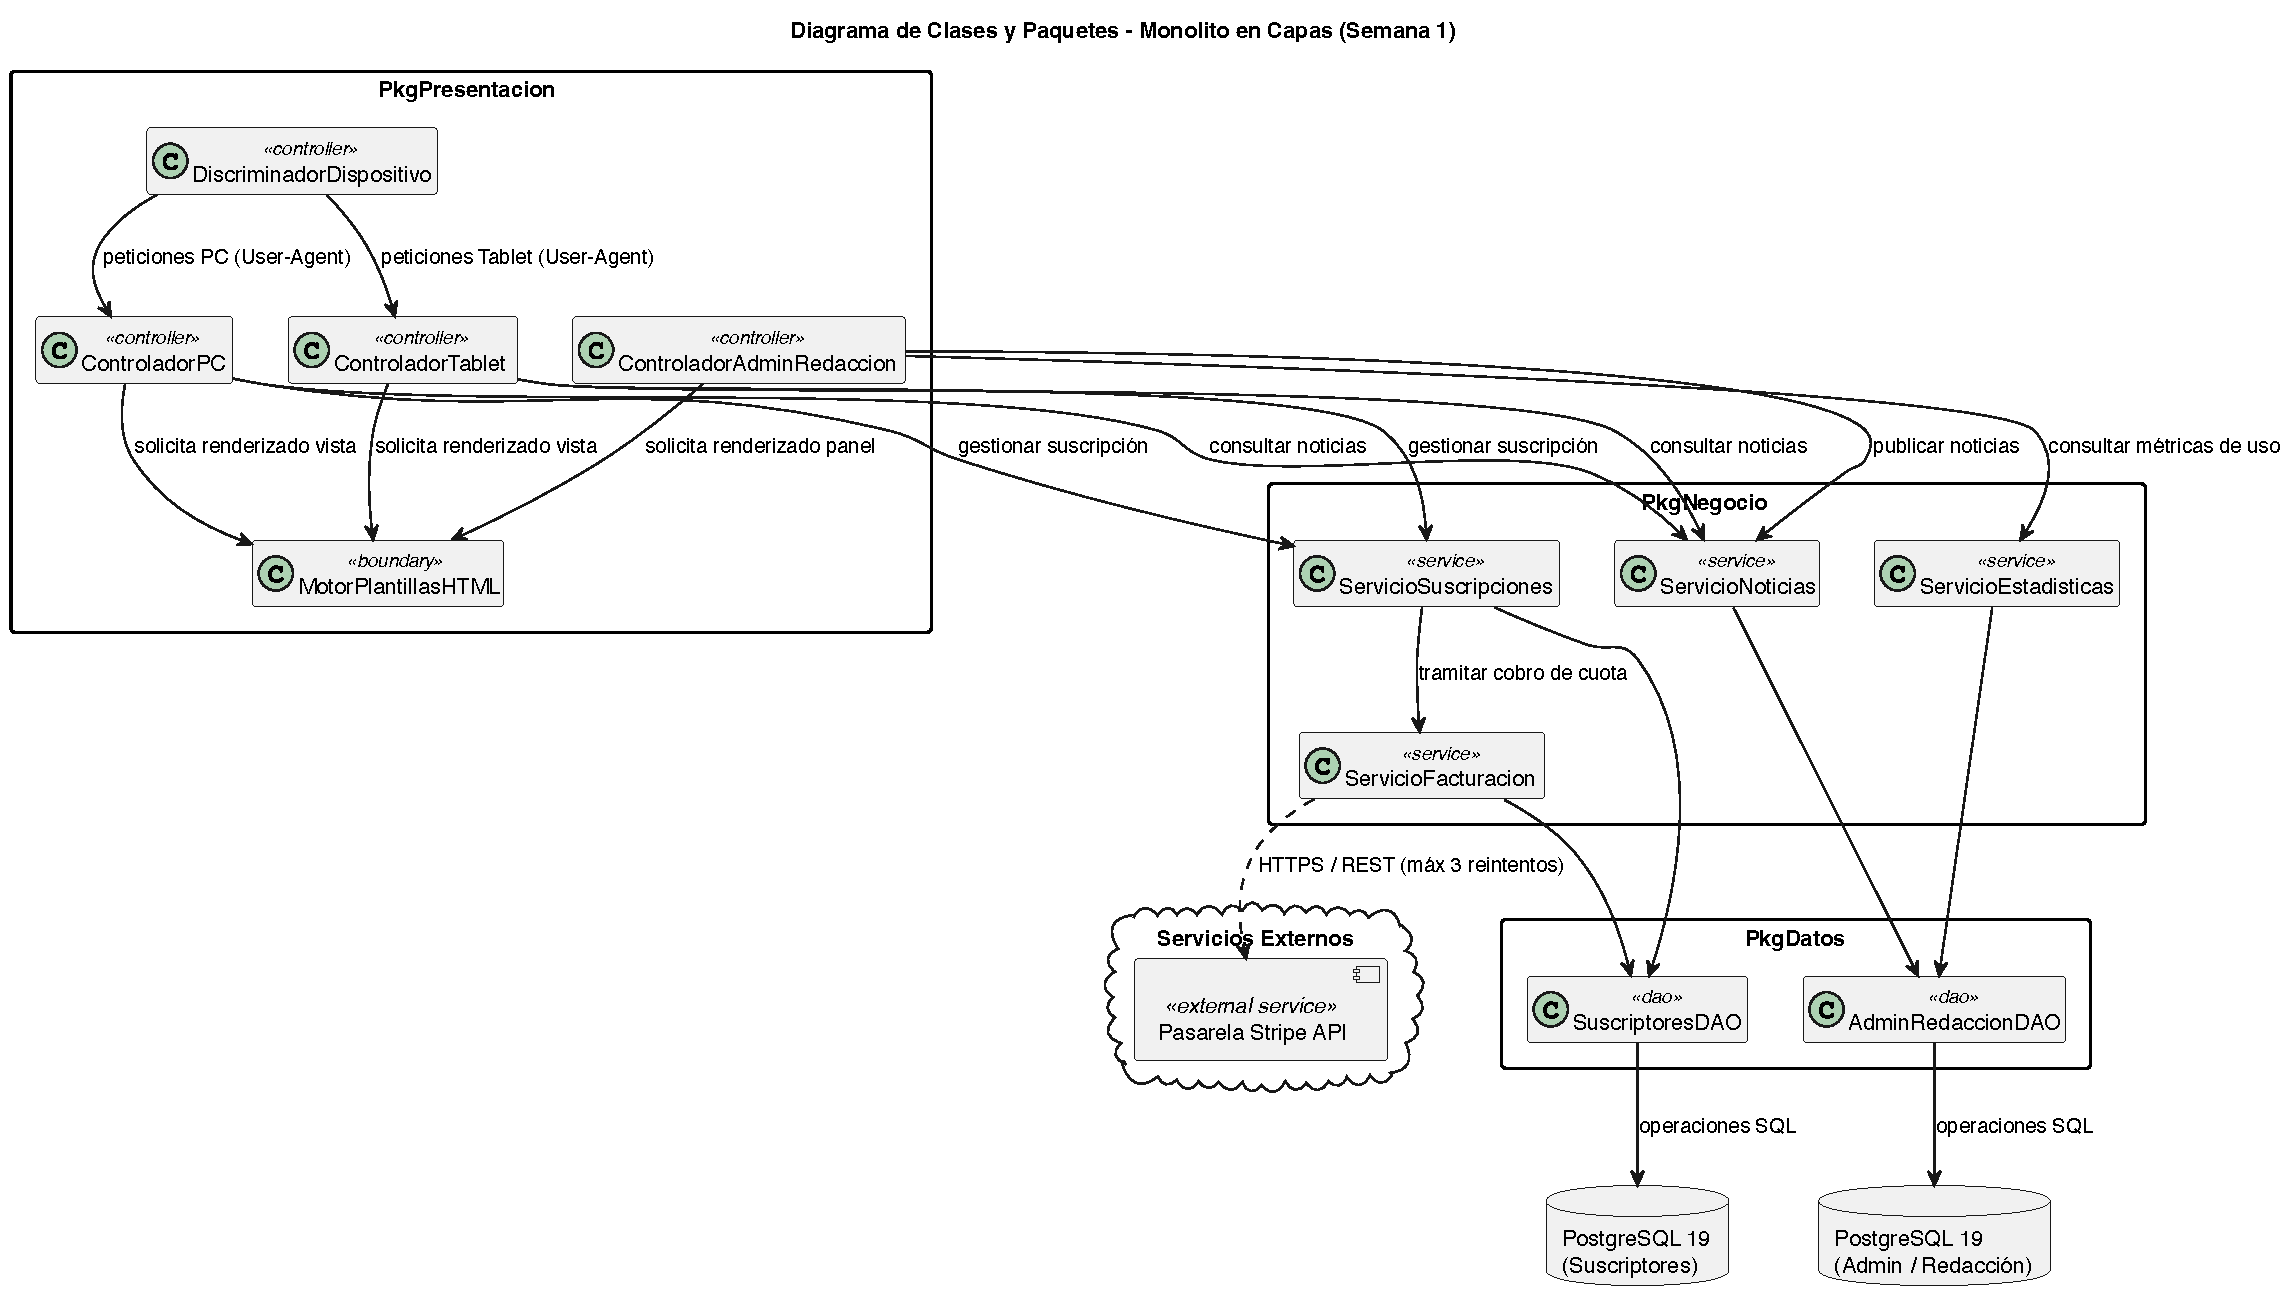
\includegraphics[width=0.9\textwidth]{assets/0001-estilo-arquitectonico-monolito-semana1.pdf}
    \caption{Primera propuesta de arquitectura monolítica.}
    \label{fig:arquitectura-monolitica}
\end{figure}

Durante la revisión del diagrama se encontraron algunos aspectos que debían corregirse. El primero estaba relacionado con la organización general del sistema. El diagrama representaba la propuesta monolítica inicial, que posteriormente fue anulada tras la discusión entre los arquitectos senior y cognitivos. Además, en esta primera representación se había incorporado un componente de base de datos antes de haber definido cómo debía organizarse el acceso a los datos.

En esta primera fase el objetivo era definir el estilo arquitectónico, por lo que todavía no era necesario entrar en tanto detalle sobre las bases de datos. Esto no significa que no deban aparecer en la arquitectura, ya que se exigen dos bases de datos PostgreSQL 19: una para administradores y redactores y otra para suscriptores.

Por tanto, el primer UML se mantiene como parte de la evolución del proyecto, aunque no representa la arquitectura finalmente seleccionada. La revisión permitió comprobar la importancia de que los componentes y las relaciones del diagrama se correspondan con las decisiones arquitectónicas tomadas.

\section{Resultado de la primera semana}

La primera semana finalizó con el análisis de requisitos mejorado y simplificado, ciñéndose a lo solicitado, y la elección de una arquitectura cliente-servidor con API REST. La propuesta monolítica inicial fue anulada después de las observaciones realizadas por los arquitectos cognitivos y de la comparación con otras alternativas. Las decisiones ADR-0001.1, ADR-0001.2 y ADR-0001.3 recogen la evolución de este primer problema de diseño.

La representación UML inicial también permitió detectar aspectos que debían revisarse antes de continuar desarrollando las clases y paquetes del sistema.

% !TEX root = ../main.tex
\chapter{Semana 2: seguimiento de la arquitectura e incorporación del API Gateway}

Durante la segunda semana se continuó desarrollando la arquitectura a partir del estilo cliente-servidor seleccionado anteriormente.

En esta fase se comenzaron a resolver problemas de diseño más concretos, relacionados con la distribución de responsabilidades entre los componentes del sistema. Una de las decisiones tratadas fue la incorporación de un API Gateway para resolver el requisito RF1, que establece que el periódico digital debe distinguir entre los clientes PC y Tablet.

\section{Decisión 0002: incorporación del API Gateway}

En la \href{Decisiones/0002.1-api-gateway-discriminacion-clientes.md}{ADR-0002.1}, los arquitectos senior propusieron incorporar un API Gateway como punto de entrada de las peticiones HTTP/REST. La finalidad de este componente era realizar la identificación del tipo de dispositivo antes de que las peticiones llegaran a los controladores del backend.

Para resolver este problema se valoraron diferentes alternativas, como realizar la identificación desde el frontend, utilizar un middleware en el backend o incorporar un API Gateway. En el caso del frontend, se podría utilizar CSS y JavaScript para adaptar la interfaz según el dispositivo, pero esto no garantiza que el backend sepa si el usuario está accediendo desde un PC o una Tablet.

Por otra parte, el middleware permitiría identificar los dispositivos directamente desde el backend, sin necesidad de añadir otro componente. Finalmente, los arquitectos senior eligieron el API Gateway porque permitía realizar esta identificación por separado, sin que los controladores del backend tuvieran que encargarse de ello.

Esta decisión fue cuestionada posteriormente por los arquitectos cognitivos, ya que se planteó si realmente era necesario añadir este componente a la arquitectura.

\section{Revisión crítica de los arquitectos cognitivos}

Durante la revisión de la decisión se cuestionó si realmente era necesario incorporar un API Gateway únicamente para distinguir entre PC y Tablet, ya que esto suponía añadir otro componente a la arquitectura del periódico.

Esta duda quedó recogida en la \href{Decisiones/0002.2-cuestionamiento-incorporacion-api-gateway.md}{ADR-0002.2}, donde se planteó si esta función podía resolverse de una forma más sencilla. Como respuesta se explicó que el profesor Rafael Capilla había recomendado utilizar un API Gateway para separar la identificación de dispositivos del backend. Además, para evitar complicar demasiado la arquitectura se decidió que el API Gateway solo tendría dos funciones: identificar si el usuario accede desde un PC o una Tablet y redirigir las peticiones HTTP/REST al controlador correspondiente. De esta forma, se mantenía la identificación de dispositivos separada del resto de funcionalidades del periódico, sin añadir más responsabilidades al API Gateway.

\section{Reafirmación de la decisión}

Después de la discusión entre los arquitectos senior y cognitivos se decidió mantener el API Gateway. Esta decisión quedó recogida en la \href{Decisiones/0002.3-reafirmacion-incorporacion-api-gateway.md}{ADR-0002.3}.

Aunque se había cuestionado su incorporación, los arquitectos senior consideraron que era una buena opción porque permitía identificar los dispositivos sin que los controladores de noticias, suscripciones y pagos tuvieran que realizar esta comprobación, aunque también se tuvieron en cuenta sus inconvenientes. Por una parte, se añadía un componente más a la arquitectura y las peticiones tenían que pasar por él antes de llegar al backend.

Finalmente, se mantuvo la decisión inicial, confirmando que el API Gateway únicamente se encargaría de identificar el dispositivo y redirigir las peticiones. Esta incorporación no supone cambiar la arquitectura cliente-servidor con API REST elegida durante la primera semana, sino añadir un componente para resolver el requisito RF1.

\section{Representación de la arquitectura en UML}

Una vez tomadas las decisiones, los arquitectos junior continuaron trabajando en el diagrama UML para representar los cambios realizados en la arquitectura.

\begin{landscape}
\begin{figure}[p]
    \centering
    \includesvg[width=0.94\linewidth]{assets/0002-estilo-cliente-servidor-rest-semana2.svg}
    \caption{Evolución de la arquitectura cliente-servidor con API REST.}
    \label{fig:arquitectura-api-rest-gateway}
\end{figure}
\end{landscape}

En este segundo diagrama se representa la separación entre el frontend y el backend, que se comunican mediante HTTP/REST. Además, se incluye el API Gateway.

Según lo establecido en la ADR-0002, el paquete \texttt{PkgApiGateway} debe contener el componente \texttt{ApiGateway} y la clase \texttt{DeviceDiscriminator}, encargada de identificar si el cliente es un PC o una Tablet. Las peticiones HTTP/REST deben pasar primero por el API Gateway y después llegar a los controladores del backend. También es importante que la identificación de dispositivos no se repita en otros componentes, ya que se ha elegido el API Gateway para encargarse de esta función. Por tanto, los arquitectos junior deben comprobar que estos elementos aparecen correctamente representados en el diagrama UML.

\section{Resultado de la segunda semana}

Durante la segunda semana se continuó desarrollando la arquitectura cliente-servidor y se tomó la decisión de incorporar un API Gateway para distinguir entre PC y Tablet. Aunque los arquitectos cognitivos cuestionaron si realmente era necesario añadir este componente, finalmente los arquitectos senior decidieron mantenerlo, limitando sus funciones para no complicar demasiado la arquitectura.

Todo este proceso quedó recogido en las ADR-0002.1, ADR-0002.2 y ADR-0002.3, donde se documentaron la decisión inicial, las dudas planteadas y su posterior verificación.


% Bibliografía desactivada temporalmente hasta su revisión.
% \clearpage
% \phantomsection
% \addcontentsline{toc}{chapter}{\bibname}
% \nocite{*}
% \bibliographystyle{plain}
% \bibliography{references}

\end{document}
